\documentclass[12pt]{report}
\usepackage{Styl}			

% Úvodní strana
\author{Daniel Sýkora}
\title{Rozšířená realita}
\date{14. února 2024}
\vedouci{Dr.rer.nat. Michal Kočer}
\place{v Českých Budějovicích}
\skolnirok{2023/2024}

\logo{
\includegraphics{GJ8_logotyp.pdf}}

\begin{document}

\mytitlepage
\prohlaseni
{
	Prohlašuji, že jsem tuto práci vypracoval samostatně s vyznačením všech použitých pramenů.
}
\abstrakt
{ % Abstrakt
	Rozšířená realita se v dnešní době stává čím dál častěji zmiňovaným tématem. \gls{xr} zařízení se stávají čím dál více dostupnějšími a v médiích často slýcháme o pojmu \textit{Metaverse} -- platformě, o kterou se technologické společnosti přou.

	Tato práce popisuje historii \gls{xr} a její různá technologická zpracování, na úrovni hardwaru i softwaru. V druhé části se zaměřuje na softwarovou stránku \gls{xr} a postup při tvorbě vlastního projektu pro \gls{vr}.
}
{ % Klíčová slova
	Headset (HMD), Rozšířená realita, Virtuální realita, Augmentovaná realita, Smíšená realita, sledování pohybu (motion tracking), herní engine
}
\podekovani
{
	Děkuji panu Michalu Kočerovi za vedení mé práce a zpětnou vazbu. Také bych rád poděkoval rodině, přátelům a spolužákům, kteří testovali můj projekt a poskytli mi na něj zpětnou vazbu.
}

\tableofcontents
\newpage

\chapter*{Úvod}
\addcontentsline{toc}{chapter}{Úvod}

Pojmem \gls{xr} (eXtended Reality; rozšířená realita) rozumíme libovolnou technologii, která nějakým způsobem upravuje realitu vnímanou člověkem. Její uplatnění je různé -- od her a virtuálních schůzek až po simulace lékařských zákroků a raketových letů. \cite{muni_kybernetika}

Nějakou formu \gls{xr} můžeme využívat na skoro každém moderním zařízení. Na mobilních zařízení augmentovanou realitu, na počítači s připojeným headsetem virtuální realitu a na speciálních samostatných (stand-alone) headsetech virtuální i smíšenou realitu. 

Tato práce popisuje historický vývoj \gls{xr} a její stav v přítomnosti. Dále popisuje technologie, které \gls{xr} aplikace využívají, po stránce hardwaru i softwaru. V praktické části se zaměřuji na \gls{vr}, s cílem vytvořit vlastní hru pro virtuální realitu za pomoci současných nástrojů.

\part{Teoretická část}

\chapter{Historie XR}

\section{Počátky XR}

První pokusy o rozšířenou realitu pochází už z 50. let 20. století, kdy Morton Hellig, americký kinematograf, přivádí na svět své zařízení zvané Sensorama. Nejednalo se ovšem o headset, které si vybavíme dnes -- Sensorama bylo stacionární zařízení, vzhledově připomínající automat. Hellig toto zařízení nazýval "zážitkovým divadlem", které bylo schopné zobrazit 3D obraz, pouštět stereo zvuk a vytvářet vítr. Tím se od dnešní XR technologie zásadně liší; nepřijímá vstup uživatele. Sensorama se ovšem nedočkala úspěchu a známe ji jen jako historicky první pokus o virtuální realitu. \cite{otechnice}

Dalším průkopníkem rozšířené reality je Ivan Sutherland, americký vědec, který je často označován jako otec počítačové grafiky. Ve svém díle The Ultimate display (ultimátní displej) popsal virtuální realitu tak, jak ji známe dnes. Virtuální realitu si představoval jako helmu, do které odesílá obraz počítač v reálném čase. Uživatel se tak měl ocitnout ve fiktivním světě nerozpoznatelným od světa reálného. \cite{otechnice} \cite{ivan_sutherland_bio}

Tuto představu se Sutherland snažil realizovat se svými studenty. Společně vynalezli vůbec první headset pro virtuální realitu, zvané The Sword of Damocles -- tedy Damoklův meč. Vzhledem k jeho primitivnosti zobrazovalo pouze čtvercové místnosti tvořené z čar, které software následně transofrmoval do správné perspektivy. Pohyby sledovalo pomocí mechanického ramene připevněného ke stropu, ze kterého byl headset zavěšený. \cite{otechnice} \cite{Rheingold_1992}

\section{XR v armádě}

V 80. letech 20. století o XR projevila zájem armáda USA, ve snaze snadněji a efektivněji připravit americké piloty na ovládání letadel. Začala využívat speciálních simulačních kabin, které obsahovaly mimo jiné i speciální headset. Tento headset pomocí stereoskopického zobrazení informoval o průběhu letu, zobrazoval 3D mapy a snímky z radaru. Díky možnosti systém ovládat pomocí hlasu nebo pohybu očí se tento headset přibližuje k dnešnímu stavu VR, jelikož reaguje na vstup uživatele. \cite{otechnice}


\begin{figure}[H]
    \centering

    \begin{minipage}{.5\textwidth}
        \centering
        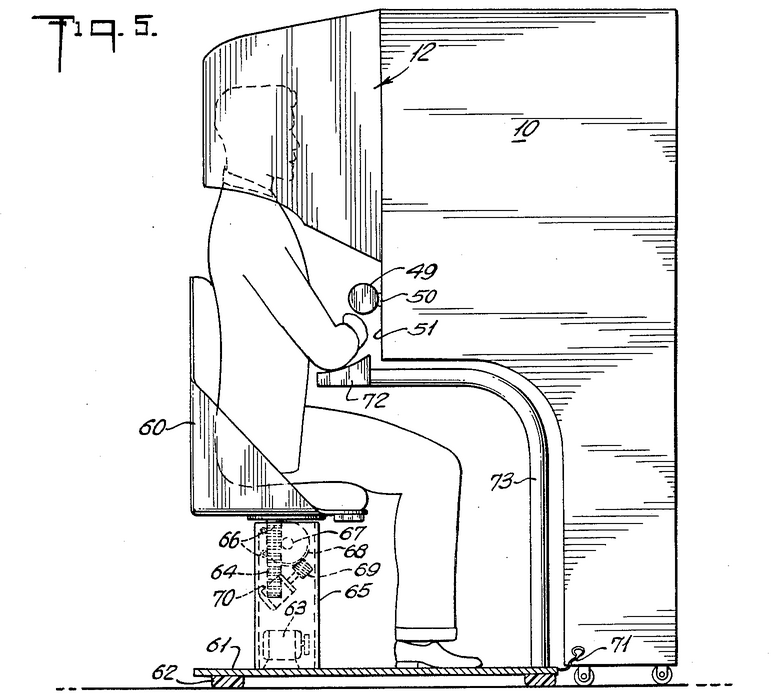
\includegraphics[height=120pt]{sensorama.png}
        \caption{Sensorama \cite{sensorama_patent}}
        \label{sensorama_fig}
    \end{minipage}%
    \begin{minipage}{.5\textwidth}
        \centering
        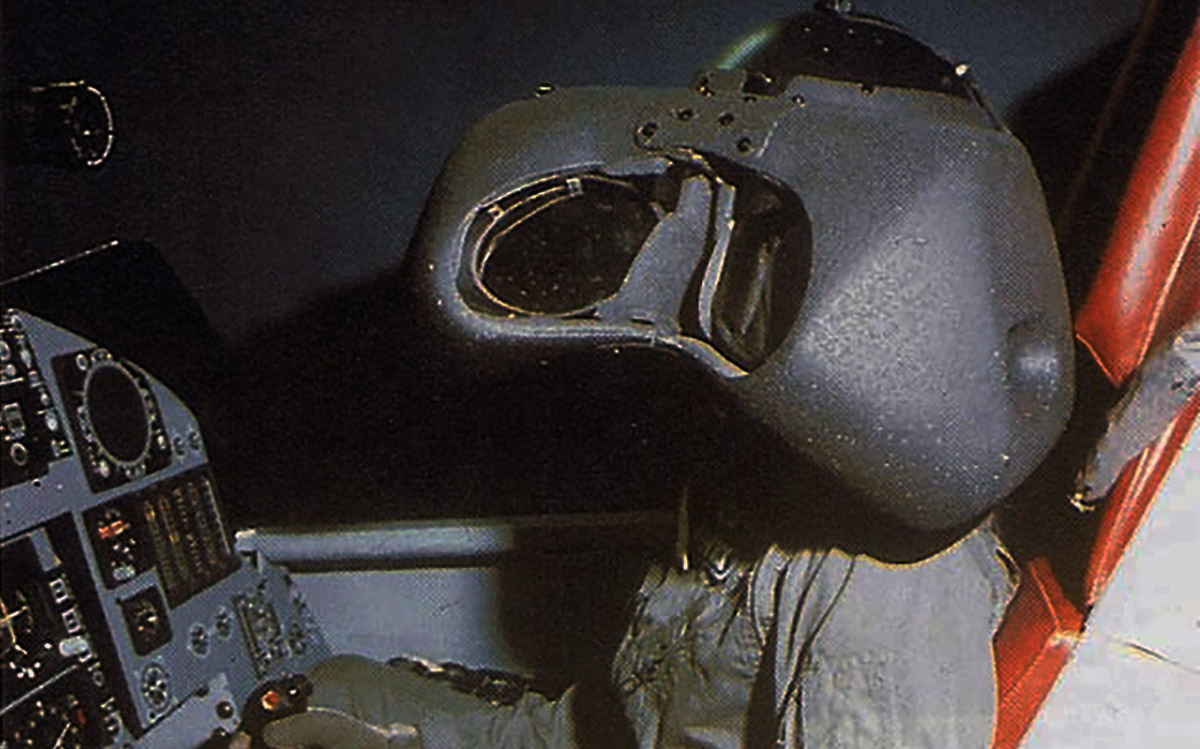
\includegraphics[height=120pt]{super_cockpit_helmet.jpg}
        \caption{Helma "Darth Vader", jedna z částí simulačního kokpitu \cite{super_cockpit_image}}
        \label{sensorama}
    \end{minipage}

\end{figure}

\section{Komerční dostupnost}

O počátku dostupnosti XR zařízení můžeme mluvit v 90. letech 20. století, kdy se tato technologie mohla dostat i do rukou obyčejných lidí. Dvojice zaměstnanců herní společnosti Atari, Jaron Lanier a Thomas Zimmermann, společně založili společnost VPL Research a začali s vývojem produktů pro XR. Zaměřili se na výrobu speciálních obleků a rukavic, které dokázaly přenést pohyby uživatele do počítače. Snímání pohybu ale nebylo dostatečně kvalitní a úspěch nezaznamenalo; dodnes je ovšem známé jako první cenově-dostupný XR systém. \cite{otechnice_2}

Herní společnosti na sebe také nenechaly dlouho čekat a začaly s vývojem VR konzolí pro hraní her. První takovou byla britská společnost Virtuality, která v roce 1991 uvedla na trh stejnojmenné zařízení představující arkádový stroj se stereoskopickými brýlemi. Kvůli vysoké pořizovací ceně nebylo dostupné pro domácnosti, Virtuality ovšem otevřela nespočet heren po celé Velké Británii. \cite{otechnice_2} \cite{independent_virtuality}

Do světa VR herních konzolí vstoupily i dnes známé japonské společnosti SEGA a Nintendo se svými SEGA VR a Virtual Boy. Obě tato zařízení však byla komerčními selháními. SEGA byla nucena kvůli technickým problémům vydání několikrát posunout a krátce po vydání skončila jeho výrobu. Nintendo sice své zařízení vydalo, ale rok po uvedení na trh jej stáhlo. Kvůli vysoké ceně a špatným grafickým schopnostem (konzole uměla zobrazit pouze červenou a černou barvu) si zálibu u hráčů nenašlo.\cite{otechnice_2}

\begin{figure}[H]
        \centering
        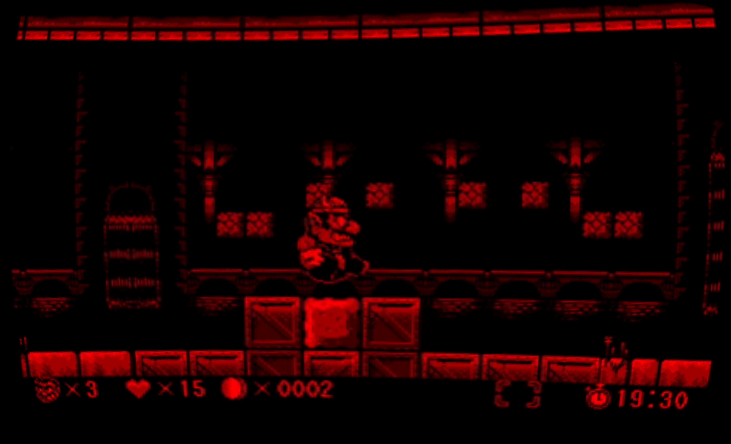
\includegraphics[height=120pt]{vboy.png}
        \caption{Červeno-černé zobrazení zařízení Virtual Boy \cite{vboy}}
        \label{vboy_red_display}
\end{figure}

\section{XR dnes}

Současná generace XR zařízení se začíná objevovat po roce 2010. Velkým průkopníkem v oblasti virtuální reality byla americká společnost Oculus, která oznámila zájem o vytvoření moderního VR systému. Jejich kickstarter\footnote{Webová stránka, kde začínající společnosti můžou žádat o finanční podporu veřejnosti. V Česku je známou alternativou \em Startovač.} se ukázal jako úspěch a přilákal pozornost jiných společností, zejména tehdejšího Facebooku (dnes Meta). Ten společnost Oculus odkoupil ještě před tím, než stačila vydat své první zařízení. Na to si zájemci museli počkat až do roku 2016, kdy bylo vydáno první zařízení zvané Oculus Rift CV1. Jeho konkurencí byl headset HTC Vive od tajwanské společnosti HTC. Tato zařízení fungovala pouze při propojení s počítačem; nebyla tedy samostatná. \cite{otechnice_3}

Vývoj mobilního VR (tedy takobho headsetu, který nepotřebuje počítač pro vykreslování obsahu) společnost Oculus konala za podpory korejského Samsungu, se kterým na trh uvedla Gear VR -- headset, který pro vykreslování používal mobilní telefon. Na podobném principu fungoval i experiment od Googlu zvaný Cardboard VR. Ten pro virtuální realitu používal pouze mobilní telefon a headset složený z kartonu (odtud název). Mobilní VR se v této době neuchytilo, zažilo ovšem velký rozmach v letech 2019-2020 po vydání headsetu Oculus Quest (dnes Meta Quest), který byl plně samostatný a používal upravenou verzi OS Android. Hry pro tento headset jsou upravené, aby běžely na Androidu, nicméně existuje možnost jej připojit k počítači a hrát hry pro "nesamostatné" headsety. \cite{otechnice_3}

Díky technologickým pokrokům a zmenšování hardwaru se také začala objevovat zařízení pro smíšenou realitu, která pomocí snímačů a pohledu z kamery umožnila vkládat virtuální předměty do reálného světa. Forem měla mnoho; například upravené optické brýle s malým displejem nebo speciální headsety. O tato zařízení se pokoušeli technologičtí giganti jako Google a Microsoft. Kvůli vysokým pořizovacím cenám ale tato zařížení u jednotlivců neuspěla a tyto společnosti s nimi dodnes cílí na pracovní prostředí. \cite{google_glass_mobilenet}

Velmi dostupné byly naopak aplikace používající augmentovanou realitu. AR byla integrována do již existujících zařízení, především jako technická dema. Běžnou metodou sledování pohybu bylo, pro svou nenáročnost, sledování speciálních předmětů či kartiček, které zařízení rozpoznalo, určilo jejich otočení a naklonění a následně zobrazilo obsah. Zlom nastal, když Google vydal ARCore, \gls{SDK} pro AR, který umožnil vývojářům sledovat pohyb mobilního telefonu pouze pomocí pohledu z kamery. Vývojáři se tím pádem mohli zaměřit pouze na vývoj jejich aplikací a her, protože nemuseli investovat čas a peníze do technologie sledování pohybu. Právě v této době vznikla většina aplikací a her, které známe. Za zmínku stojí například Pokémon GO. \cite{enwiki:1182789097}

\chapter{Hardware}
lorem ipsum

něco o trackování, výrobcích, atd. zmínit trackovací systém bez věží od Meta/FB

\section{Degrees of freedom}

Degrees of freedom (DoF), česky \em{stupně volnosti}, označuje směry v prostoru ve kterých je sledován pohyb. V oblasti XR rozlišujeme pojem 3DoF a 6DoF. Systém, který sleduje pohyb ve 3DoF sleduje pouze náklon zařízení. Umožňuje tím např. rozhlížet se; dívat se jinými směry. Systém, který sleduje pohyb v 6DoF je dále schopný sledovat pohyb dopředu/dozadu, doleva/doprava a nahorů/dolů. Umožňuje tak se pohybovat ve virtuálním prostoru. 

\chapter{Software}
lorem ipsum

zmínit OpenXR, WebXR jakožto API co pohánějí XR

rozlišit PCVR na windows a mobilní VR na bázi androidu
\part{Praktická část}

\chapter{Cíl projektu}

V praktické části mé práce jsem vytvořil vlastní hru pro VR. Stanovil jsem si následující kritéria:

\begin{itemize}
  \item \textbf{Nenáročnost}. Chtěl jsem, aby má hra nebyla obtížná na pochopení. Většina VR her vyžaduje zvýšenou fyzickou aktivitu nebo hlubší porozumění VR konceptů. Ideálně jsem chtěl vytvořit hru, kterou bych mohl komukoliv půjčit, aniž bych musel dlouze vysvětlovat její princip.
  \item \textbf{Grafická jednoduchost}. Nepovažuji se za umělce a umím vytvářet pouze základní modely a textury. Bylo pro mě tedy klíčové přijít s takovým konceptem, který by byl vzhledově nenáročný.
  \item \textbf{Interaktivita}. Od své hry jsem chtěl, aby doopravdy využívala funkce, které VR platformy poskytují. Tedy ovládání pohybem, vliv fyzikálních zákonů atp.
\end{itemize}

\begin{quotation}
  
\textbf{Dospěl jsem k následujícímu nápadu}: Logická hra sestávající z kostky tvořené úrovněmi naskládanými na sebe. Každá úroveň představuje bludiště, skrze které musí nakláněním hráč navigovat kuličku. Při dosažení cíle je úroveň odebrána, kostka se zmenší a je odhalena další úroveň.
\end{quotation}

Toto splňuje moje kritéria -- hra je jednoduchá, na vykreslení potřebuje jen geometrické tvary a vyžaduje pohyb rukama pro naklánění bludiště.

Výsledný projekt je složen z mnoha souborů, mnoho z nichž nejsou kód a není vhodné je do textu práce zahrnout. 

Celý zdrojový kód je veřejnosti dostupný na adrese \url{https://github.com/sykdan/puzzle_prism/tree/mprace}. 

\chapter{Struktura projektu}

\begin{samepage}
  Můj projekt jsem rozdělil do jednotlivých, jednoduše spravovatelných scén. Tímto jsem mohl na mnohých funkcích pracovat odděleně a mohl bych je teoreticky použít i v budoucích projektech. Zde je zjednodušený diagram těchto scén:

  \vspace{1em}
  \hrule
  \vspace{1em}

  \renewcommand\DTstyle{\sffamily}
  \dirtree{%
    .1 Hlavní scéna (spojuje a ovládá zbylé scény) .
    .2 Prostředí (skybox) .
    .2 Hráč .
    .3 Trackované ovladače, kamera synchronizovaná s headsetem .
    .2 Obrazovka .
    .3 Výběr obtížnosti, žebříček nejlepších, nastavení hry .
    .2 Kostka s bludištěm .
    .3 Kostka o určité velikosti .
    .4 Úroveň (bludiště, ze kterých se kostka skládá) .
    .5 Komnata (buňky, ze kterých se skládá bludiště) .
    .3 Kulička (volně se pohybující předmět s vlastní fyzikou) .
  }
  \vspace{1em}
  \hrule
  \vspace{1em}

  Každá scéna reprezentuje odlišnou sadu problémů a výzev, které jsem musel při tvorbě projektu řešit.
\end{samepage}

\section{Hráč, interakce se zařízením}

Scéna s hráčem je přímo spojena s headsetem a sledovanými ovladači. Sestává z uzlů \texttt{XRCamera3D}, pohledu do 3D prostředí synchronizovaným s umístěním headsetu, a dvou uzlů \texttt{XRController3D}, které jsou synchronizované s umístěním levého a pravého ovladače.

V této scéně jsem použil svobodnou knihovnu \textit{Godot XR Tools}, která nabízí podpůrné scény pro XR projekty. Z té jsem si zapůjčil kód nutný k inicializaci VR headsetu a 3D model ruky licencovaný pod \textit{Creative Commons 0}\footnote{CC0 je licence používaná pro díla ve veřejné doméně. Autoři modelu se vzdali autorských práv. Vizte \url{https://creativecommons.org/publicdomain/zero/1.0/deed.cs}}.

Od přátel, kteří hru testovali, jsem často slýchal stížnosti, že jim hra způsobuje nevolnost. Přidal jsem proto do této scény i platformu, umístěnou pod hráčem ve výšce, kterou si ve svém zařízení předem nastavil jako výšku podlahy. Mým záměrem bylo zabránit pocitu, že se hráč \uv{vznáší v prázdnotě}, čímž bych nepříjemný pocit odstranil. Testující na změnu reagovali pozitivně. 

Účel scény je kromě správného zobrazení hry také interpretace vstupu od hráče. Ve hře jsou klíčové dvě funkce: uchopení nějakého předmětu (např. kostky pro její naklánění) a interakce s uživatelským rozhraním pomocí laserového ukazovátka. Druhý zmíněný bod popisuji podrobněji v sekci \ref{uzivatelske_rozhrani}.

Implementovat uchopení předmětu \textit{jednou rukou} je triviální -- Stačí, aby tento objekt sledoval změny v transformaci uzlu \texttt{XRController3D}. Uchopení \textit{oběma rukama}, chování, kterého jsem chtěl dosáhnout ve své hře, je ale složitější. Protože je možné ovladače volně pohybovat a neexistují žádná fyzická omezení (hráč by mohl předmět např. volně kroutit), musel jsem přistoupit ke kompromisu. Při sevření tlačítek na obou ovladačích hra vytvoří třetí, neviditelný ovladač. Tento ovladač působí ze středu mezi levým a pravým ovladačem a je rotován tak, aby vektor Z tranformační matice\footnote{Godot Engine používá pro rotaci uzlů transformační matice. Vektor Y míří vzhůru.} mířil od levého ovladače k pravému ovladači a vektor Y mířil stejným směrem jako palce uživatele. Hra se poté odkazuje na tento virutální ovladač. Výsledný efekt je velmi přesvědčivý. Celá implementace této logiky je vložena v příloze \ref{apx_gripped_object_transformation}.

\section{Kostka, bludiště}

Kostka je hlavním prvkem hry. Jedná se o dutou kostku s průhledným víkem, ve které je několik úrovní (bludišť) a kulička. Každé bludiště je v podstatě mřížka čtvercových buněk, které jsou odděleny zdmi. Cílem je manipulováním s kostkou dostat kuličku k vlajce, načež kulička propadne o úroveň níž a kostka se zmenší.

Hlavní výzvou v této scéně je vygenerování náhodného bludiště, aby bylo možné hru hrát donekonečna.

\begin{figure}[H]
  \centering
  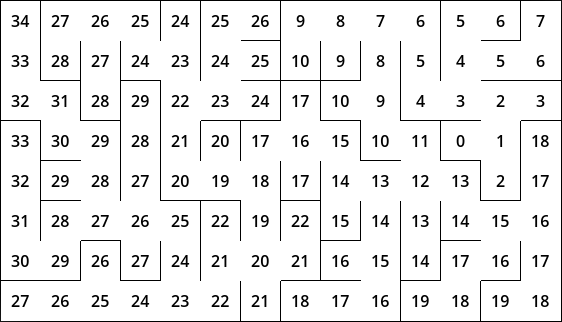
\includegraphics[height=180pt]{maze_example.png}
  \caption{Ukázka vygenerovaného bludiště (v 2D podobě) z testovací scény}
  \label{maze_example}
\end{figure}

Pro vygenerování bludiště jsem použil \textit{\textbf{Wilsonův algoritmus}}. Důvodem je fakt, že tento algoritmus nemá sklony vytvářet extrémně dlouhé či extrémně krátké chodby, na rozdíl od jiných algoritmů. Postup je následující: \cite{enwiki:1193338583}

\begin{enumerate}
  \setcounter{enumi}{0}
  \item Mějme graf buněk, kde má každá buňka několik sousedních buněk (např. pro mřížku mají buňky 4 sousední buňky, vyjma těch na krajích a v rozích). Nechť je mezi všemi sousedícími buňkami spojení, které lze označit jako průchod nebo zeď.
  \item Označme všechny spojení jako zdi a jednu náhodně zvolenou buňku označme jako zahrnutou v bludišti. \label{init}
  \item Libovolným způsobem zvolme buňku. Pokud je tato buňka zahrnuta v bludišti, zvolme jinou buňku. \label{pick}
  \item Označme buňku jako zahrnutou v současné iteraci.
  \item Přejděme na náhodnou sousedící buňku a v předchozí buňce uložíme ukazatel k následující buňce. Poté: \label{lerw}
        \begin{itemize}
          \item Pokud tato buňka není zahrnuta ani v iteraci, ani v bludišti, označme ji jako zahrnutou v iteraci a přejděme na krok \ref{lerw}.
          \item Pokud je tato buňka zahrnuta v iteraci, vznikla smyčka. Pomocí ukazatelů uložených v buňkách projděme tuto smyčku, odstraňme buňky ze současné iterace a odeberme ukazatele.
          \item Pokud je tato buňka zahrnuta v bludišti, všechny buňky v iteraci označme jako buňky v bludišti. Spoje mezi buňkami v této iteraci označme jako průchody.
        \end{itemize}
  \item Pokud stále existují buňky, které nejsou zahrnuty v bludišti, přejděme zpět ke kroku \ref{pick}.
\end{enumerate}

\begin{figure}[H]
  \centering

  \begin{minipage}{.5\textwidth}
    \centering
    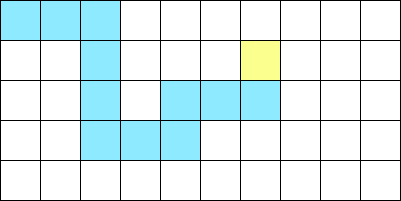
\includegraphics[height=100pt]{maze_gen_step_1.png}
  \end{minipage}%
  \begin{minipage}{.5\textwidth}
    \centering
    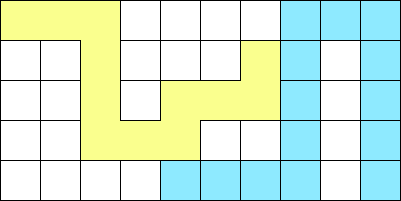
\includegraphics[height=100pt]{maze_gen_step_2.png}
  \end{minipage}

  \caption{Příklad dvou iterací kroků \ref{pick} až \ref{lerw}. Žlutě jsou zvýrazněny buňky v bludišti, modře buňky v iteraci.}
\end{figure}

\begin{figure}[H]
  \centering
  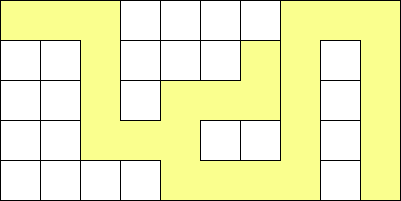
\includegraphics[height=120pt]{maze_gen_step_3.png}
  \caption{Stav po těchto dvou iteracích}
\end{figure}

Takto vygenerované bludiště nemá žádný začátek ani konec; je stvořené z náhodně propletených buněk. V prvních verzích hry byl konec náhodně zvolený, docházelo ale k situacím, kdy byl konec velmi blízko počáteční pozici. Algoritmus jsem proto upravil, aby zároveň zaznamenával vzdálenost od úvodní buňky (viz krok \ref{init}). Jelikož výběr úvodní buňky nemá na výsledek algoritmu vliv, umožnil jsem explicitně zadat její pozici. Úvodní buňku teď můžu považovat za začátek bludiště, a nejvzdálenější buňku jako konec. Celá implementace algoritmu je uvedena v příloze \ref{apx_mazegen}.

\begin{figure}[H]
  \centering

  \begin{minipage}{.5\textwidth}
    \centering
    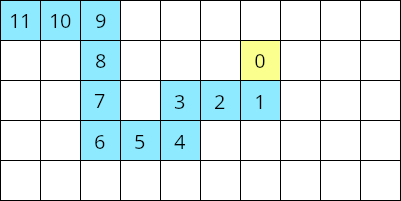
\includegraphics[height=100pt]{maze_gen_count_1.png}
  \end{minipage}%
  \begin{minipage}{.5\textwidth}
    \centering
    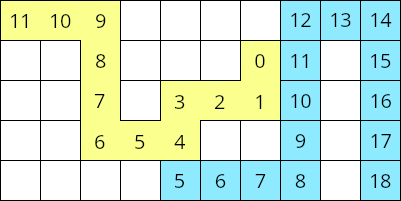
\includegraphics[height=100pt]{maze_gen_count_2.png}
  \end{minipage}

  \caption{Počítání vzdálenosti paralelně s generováním}
\end{figure}

Po vygenerování bludiště hra podle výsledných dat postaví bludiště. Instancuje scénu s úrovní a v jednotlivých komnatách připraví zdi. Aby se zabránilo dlouhým načítacím dobám, lze hru hrát již po vygenerování dvou úrovní. Zbytek je generován a doplněn na pozadí, předpokládá se, že hráč bude hrát pomaleji, než se hra generuje.

Druhou výzvou je samotná fyzika kuličky. Godot Engine nabízí modul pro simulaci fyziky, kterého jsem využil. Kuličku tvoří uzel \texttt{RigidBody3D} (tuhé těleso) a stěny uzel \texttt{StaticBody3D} (nehybné těleso). Fyzika je následně procesována automaticky. Přidal jsem však haptickou odezvu při srážce kuličky se stěnou bludiště -- při prudké změně v rychlosti kulička vyšle signál se sílou vibrace, který hlavní scéna zaznamená a ve scéně s hráčem vyvolá slabou vibraci v ovladačích.

\begin{figure}[H]
  \centering
  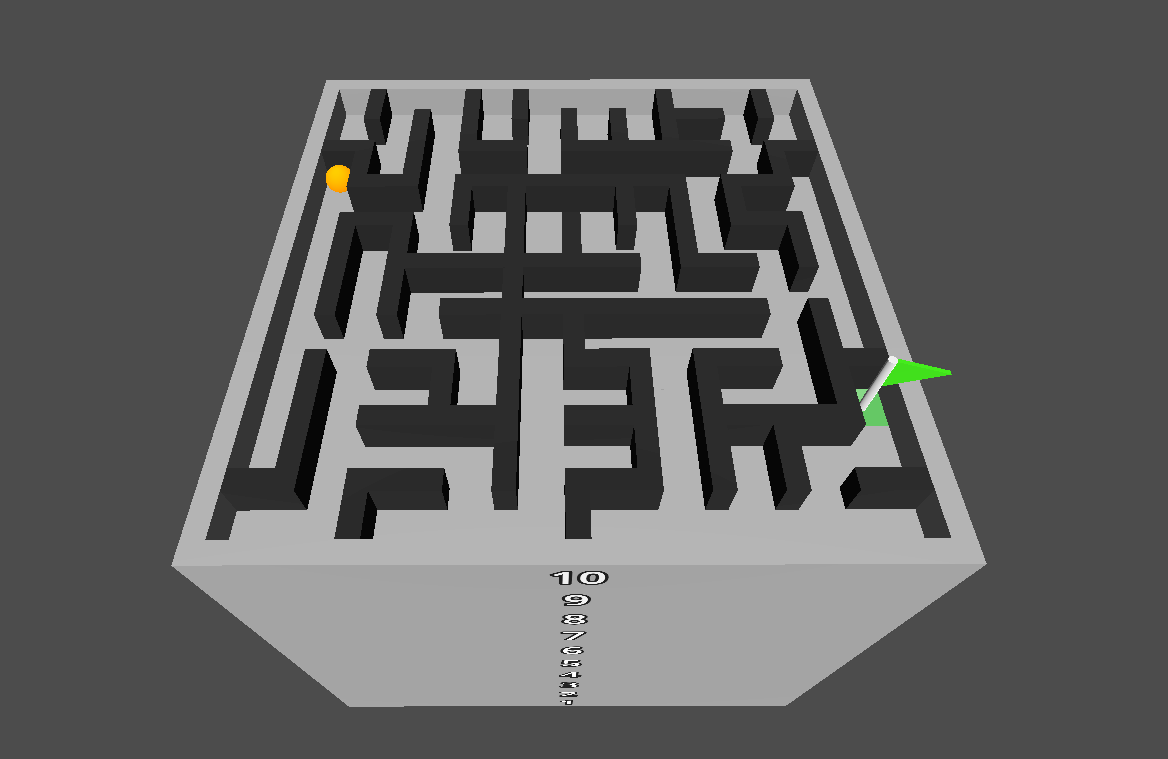
\includegraphics[height=180pt]{maze.png}
  \caption{Celá kostka}
  \label{maze_fig}
\end{figure}

\label{uzivatelske_rozhrani}
\section{Uživatelské rozhraní}

Grafické uživatelské rozhraní je nedílnou součástí každé aplikace nebo hry. Ve VR ovšem nemáme k dispozici myš ani klávesnici, vše je ovládáno pohybem. Přesto je ale možné dosáhnout podobného chování, jaké známe z tradičních rozhraní. Většina VR softwaru používá pro své rozhraní virtuální \uv{obrazovky}, plošiny, které zobrazují 2D obsah podobně jako monitor. Uživatel poté využívá virtuální \uv{laserové ukazovátko}, kterým na tyto obrazovky ukazuje a stisknutím tlačítka s nimi interaguje.

\begin{figure}[H]
  \centering
  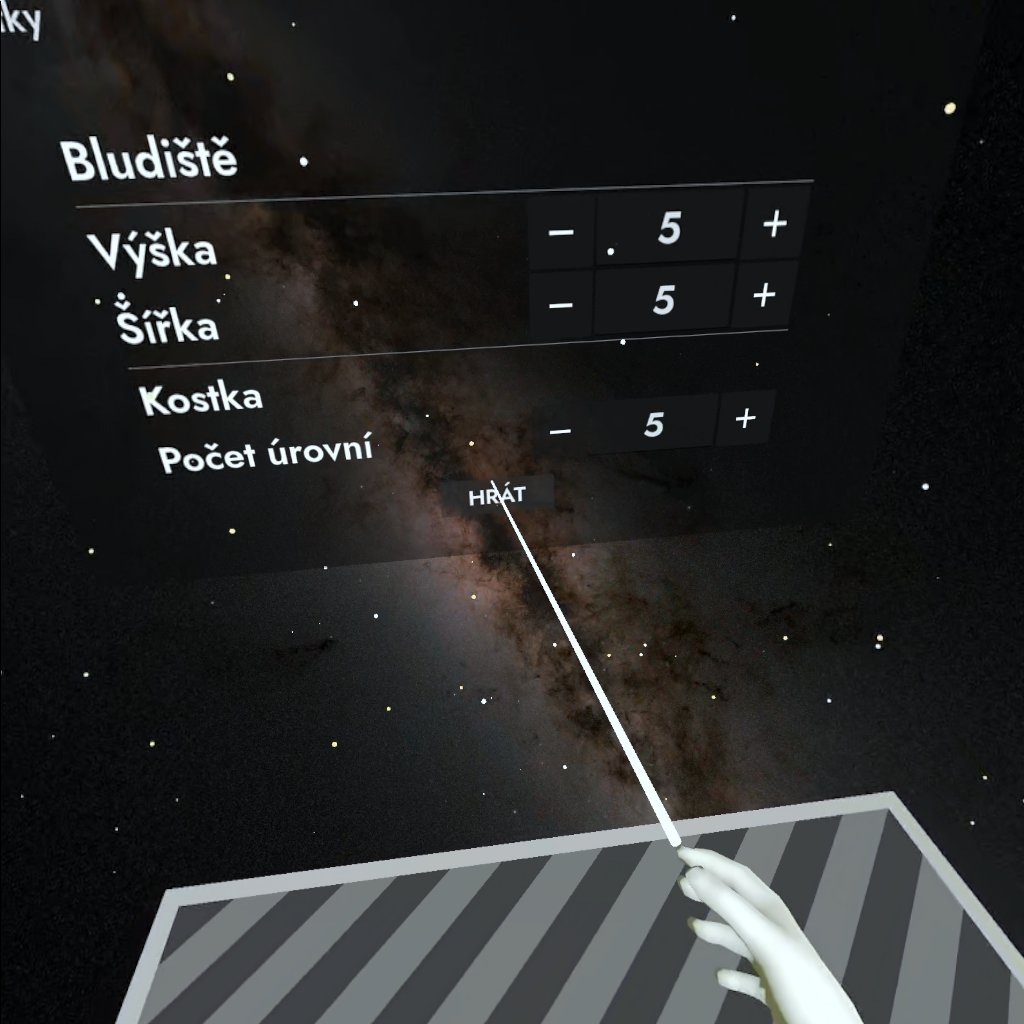
\includegraphics[height=220pt]{game_gui_screenshot.png}
  \caption{Ukázka rozhraní hry. Uživatelova pravá ruka je vybavena ukazovátkem, kterým může vybírat možnosti na obrazovce.}
  \label{game_gui_screenshot}
\end{figure}

Pro vykreslení orbazovky jsem použil uzel \texttt{SubViewport}, který umožňuje vytvořit virtuální plátno a libovolně ho v rámci enginu zobrazit. Tomuto uzlu můžu přiřadit libovolné dceřinné uzly, které jsou poté renderovány do tohoto plátna. Samo o sobě není vidět, ale může být přiřazeno jako textura k jinému uzlu. Pro můj účel jsem použil uzel \texttt{MeshInstance} (instance 3D objektu) a jako objekt použil jednoduchý obdélník.

Interakce s obrazovkou využívá postup zvaný \textit{ray casting}, česky \textit{vysílání paprsků}. Z ruky hráče vyšleme paprsek směrem, kterým ukazuje, a při kolizi s nějakým objektem (v tomto případě obrazovkou) vypočítáme pozici, kde ke kolizi došlo. Godot Engine má podporu pro ray casting v rámci uzlu \texttt{RayCast3D}, který jsem přidal do scény s hráčem. Pokud tento uzel zaznamená kolizi se scénou Obrazovka, zobrazí paprsek mířící od prstu hráče k obrazovce a začne v jejím \texttt{SubViewport}u simulovat vstup myší. Simulování vstupu mi umožňuje využít nespočet vestavěných uzlů pro tvorbu rozhraní.

\chapter{Scénář hry}

Při vstupu do hry se hráč ocitne v hlavní nabídce. Ta je koncipovaná co nejjednodušeji - hráči jsou ihned představeny čtyři herní režimy, stupňované dle komplexity.

\begin{itemize}
  \item \textbf{Lehká obtížnost} - Bludiště má rozměry 5x5 buněk a kostka má 5 úrovní.
  \item \textbf{Střední obtížnost} - Bludiště má rozměry 8x8 buněk a kostka má 8 úrovní.
  \item \textbf{Těžká obtížnost} - Bludiště má rozměry 14x14 buněk a kostka má 14 úrovní.
  \item \textbf{Vlastní} - Hráč si může volně přizpůsobit rozměry hry.
\end{itemize}

K dispozici jsou i menší, méně důležitá tlačítka pro vstup do nastavení, ukončení hry a zobrazení návodu. Návod se hráči otevře také při úplně prvním spuštění hry.

U všech režimů hra zaznamenává čas, za jaký byl hráč schopný hlasvolam vyřešit. Přednastavené obtížnosti (lehká, střední, těžká) taktéž ukládají pět nejlepších výsledků. Pokud hráč pokoří jeden z těchto rekordů, dostane možnost zadat své jméno a uložit tím svůj čas. 
\chapter*{Závěr}
\addcontentsline{toc}{part}{Závěr}

\lipsum[1]

\nocite{*}

\addcontentsline{toc}{part}{Přílohy}
\addcontentsline{toc}{chapter}{Bibliografie}
\printbibliography

\setglossarystyle{list}
\printglossary[title={Zkratky}]

\listoffigures
\addcontentsline{toc}{chapter}{\listfigurename}

\appendix

\chapter{Základní ukázka GDScript kódu}\label{apx_gscript_sample}
\lstinputlisting{code/sample_gdscript.gd}

\chapter{Ovládání pohybem obou rukou}\label{apx_gripped_object_transformation}
Tento kód z velké části využívá faktu, že uzly v Godotu dědí své transformace. Pokud se pohne rodičovský uzel, dceřinný uzel se pohne společně s ním, a rozdíl pozice a rotace mezi nimi zůstane stejný. Toto chování je ovšem ignorováno v instrukcích, které mění hodnoty atributů \texttt{global\_*}.

Většina pohybem ovládaných uzlů má proto jeden dceřinný uzel (v kódu nazván jako \textit{Origin}), který je při uchopení přemístěn úpravou \texttt{global\_transform} tak, aby umístěním splýval s uchyceným předmětem (toto v přiloženém kódu není obsaženo). Uchycený předmět je poté synchronizován s pozicí a rotací tohoto \textit{Origin}u. Není tak potřeba manuálně počítat rozdíl transformace.

\lstinputlisting{code/gripped_object_transformation.gd}

\chapter{Wilsonův algoritmus v GDScript}\label{apx_mazegen}
\lstinputlisting{code/mazegen.gd}

\chapter{Snímky ze hry}

\end{document}
